%!TEX root = informe.tex
\chapter{Análisis de Ciclo de Vida: instalación}
\section{Capas componentes}

(Fuente: Manual Técnico para la correcta colocación de los Euroadoquines (MTCE 04))

\begin{itemize}
\item Explanada: Terreno natural adecuadamente compactado hasta alcanzar una capacidad portante mínima.
\item Subbase: Conjunto de capas naturales, de material granular seleccionado, estabilizado y compactado, situadas directamente sobre la explanada.
\item Base: Principal elemento portante de la estructura, situada sobre la subbase. Puede ser realizada con material granular, zahorra artificial, con un mayor grado de compactación que el alcanzado en la subbase (Base Flexible), o estar realizada con hormigón magro (Base Rígida).
\item Lecho de árido: Base de apoyo de los adoquines, destinada a absorber sus diferencias de espesor debidas a la tolerancia de fabricación, de manera que estos una vez compactados formen una superficie homogénea.
\item Adoquines: Elementos prefabricados de hormigón, cuya cara exterior, una vez colocados, forman la capa de rodadura de la superficie a pavimentar.
\item Relleno final: Una vez encastrados en el lecho de árido, sus juntas precisan un relleno final para transferir a los elementos contiguos las cargas a las que sean sometidos por acción del tráfico.
\end{itemize}

\section{Determinación de la sección tipo}\label{sec:secciontipo}

Se consideran los siguientes casos:

\begin{enumerate}
\item Viales y zonas de aparcamiento\footnote{No suelen existir zonas peatonales puras (paso eventual de vehículos de mantenimiento, limpieza y servicios).}.
\item Zonas industriales.
\end{enumerate}


Para cada caso, viales o zonas industriales, la sección puede obtenerse de forma abreviada en función de dos variables:
\begin{itemize}
\item Tipo de explanadas.
\item Categoría de tráfico.
\end{itemize}

\subsection{Tipo de explanada}

Se utiliza un sistema de clasificación de su capacidad portante mediante el índice CBR (California Bearing Ratio), indicando el tanto por ciento de la presión ejercida por un pistón sobre el suelo para alcanzar una determinada penetración baremado según un juego de muestras normalizados (ver tabla \ref{indicecbr}.

\begin{table}[!htb]
\centering
\begin{tabular}{|c|c|}
\hline
Calidad de la explanada & Índice CBR\\ \hline
E1 & 5 $\leq$ CBR = 10\\ \hline
E2 & 10 $\leq$ CBR = 20\\ \hline
E3 & 20 $\leq$ CBR\\ \hline
\end{tabular}
\caption{Índice CBR.}
\label{indicecbr}
\end{table}


\subsection{Categoría de tráfico}

\begin{table}[!htb]
\centering
\begin{tabular}{|c|c|}
\hline
Tipo & Categoría de tráfico\\ \hline
Viales y zonas de aparcamiento & C0 \ldots C4\\ \hline
Zonas industriales & A \ldots D\\ \hline
\end{tabular}
\caption{Categoría de tráfico.}
\label{categoriadetrafico}
\end{table}

\subsubsection{Categorías de tráfico en viales y zonas de aparcamiento}

Si en un área limitada existen diversos usos, a efectos de unificación se debería emplear para toda la zona la carga de cálculo más exigente.

\begin{table}[!htb]
\centering
\begin{tabular}{|p{7cm}|c|}
\hline
\centering{Uso previsto} & Categoría de tráfico\\ \hline
Arterias principales con gran afluencia de tráfico, paradas de bus, estaciones de servicio, etc. (50 a 149 v.p.d.) & C0\\ \hline
Arterias principales (25 a 49 v.p.d.) & C1\\ \hline
Calles comerciales con gran actividad (16 a 24 v.p.d.) & C2\\ \hline
Calles comerciales cone escasa actividad (15 v.p.d.) & C3\\ \hline
Áreas peatonales, calles residenciales & C4\\ \hline
\end{tabular}
\caption{Categoría de tráfico en viales y zonas de aparcamiento.}
\label{categoriadetraficoenviales}
\end{table}


\subsubsection{Categorías de tráfico en zonas industriales}

\begin{table}[!htb]
\centering
\begin{tabular}{|c|c|c|c|}
\hline
\multicolumn{2}{|c|}{Área} & Uso & Intensidad de uso\\ \hline
\multirow{7}{*}{Comercial} & De operación &  & Alta\\ \cline{2-4}
& \multirow{2}{*}{Almacenamiento} & Mercancia convencional & Media\\ \cline{3-4}
& & Mercancía pesada & Alta\\ \cline{2-4}
& Manipulación & & Alta\\ \cline{2-4}
& \multirow{3}{*}{Estacionamiento} & Vehículos pesados y ligeros & Media\\ \cline{3-4}
& & Vehículos pesados exclusivamente & Alta\\ \cline{3-4}
& & Semirremolques & Alta\\ \hline
\multirow{3}{*}{Militar} & De operación &  & Alta\\ \cline{2-4}
& \multirow{2}{*}{Almacenamiento} & Mercancia convencional & Media\\ \cline{3-4}
& & Mercancía pesada y semirremolques & Alta\\ \hline
\multirow{3}{*}{Pesquera} & Almacenamiento &  & Media\\ \cline{2-4}
& Manipulación & & Alta\\ \cline{2-4}
& Clasificación y venta & & Media\\ \hline
\multirow{3}{*}{Industrial} & De operación &  & Alta\\ \cline{2-4}
& \multirow{2}{*}{Almacenamiento} & Mercancia convencional & Media\\ \cline{3-4}
& & Mercancía pesada & Alta\\ \hline
\end{tabular}
\caption{Intensidades de uso en zonas industriales.}
\label{categoriadetraficoenzonasindustrialesintensidades}
\end{table}


\begin{table}[!htb]
\centering
\begin{tabular}{|c|c|c|c|}
\hline
\multirow{2}{*}{Intensidad de uso} & \multicolumn{3}{c|}{Carga de cálculo} \\ \cline{2-4}
 & Alta & Media & Baja\\ \hline
Elevada & A & B & C\\ \hline
Media & A & B & D\\ \hline
Reducida & B & C & D\\ \hline
\end{tabular}
\caption{Categoría de tráfico en zonas industriales.}
\label{categoriadetraficoenzonasindustriales}
\end{table}

\section{Secciones tipo}

Las secciones tipo según la base y el uso previsto del área vistas en la sección \ref{sec:secciontipo} pueden resumirse en cinco tipos para cada tipo de base, granular (figura \ref{fig:seccionestipogranular}) u hormigón magro (figura \ref{fig:seccionestipohormigon}).

\begin{figure}[!htb]
\centering
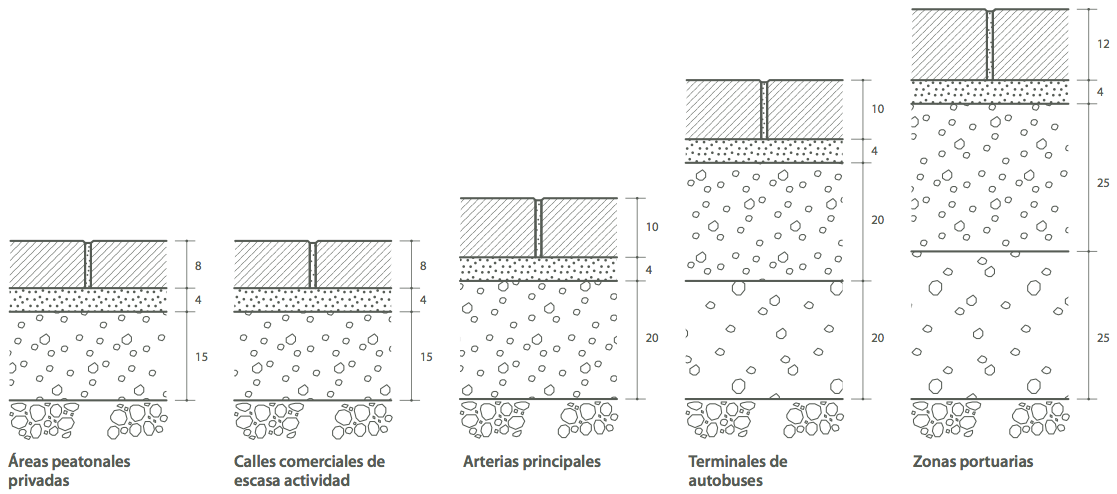
\includegraphics[width=15cm]{seccionestipo_1.png}
\caption{Secciones tipo para base granular. Unidades en cm.}
\label{fig:seccionestipogranular}
\end{figure}

\begin{figure}[!htb]
\centering
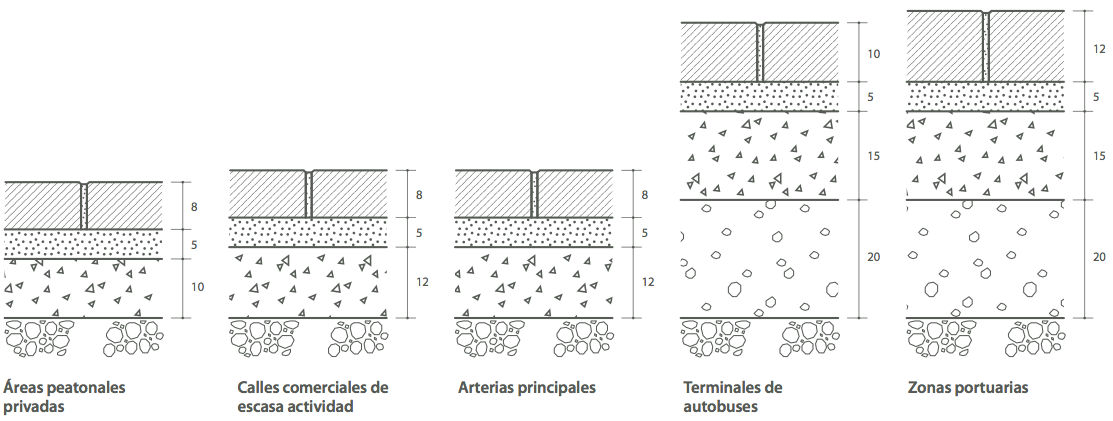
\includegraphics[width=15cm]{seccionestipo_2.png}
\caption{Secciones tipo para base de hormigon. Unidades en cm.}
\label{fig:seccionestipohormigon}
\end{figure}
